\documentclass[conference]{IEEEtran}
\IEEEoverridecommandlockouts

\usepackage{cite}
\usepackage{amsmath,amssymb,amsfonts}
\usepackage{algorithmic}
\usepackage{graphicx}
\usepackage{textcomp}
\usepackage{xcolor}
\usepackage{booktabs}
\usepackage{multirow}
\usepackage{url}

\def\BibTeX{{\rm B\kern-.05em{\sc i\kern-.025em b}\kern-.08em
    T\kern-.1667em\lower.7ex\hbox{E}\kern-.125emX}}

\begin{document}

\title{iDEFT: Intelligent Backup-Node Selection for\\ Fault-Tolerant Network Function State Replication}

% \author{
% \IEEEauthorblockN{Your Name\IEEEauthorrefmark{1}}
% \IEEEauthorblockA{\IEEEauthorrefmark{1}Department of Computer Science and Engineering, Your University\\
% Email: your.email@example.edu}
% }

\maketitle

\begin{abstract}
Network Function Virtualization (NFV) systems that provide fault tolerance through
state replication (OpenNF, Pico Replication, FTMB, REINFORCE, and DEFT among them)
all replicate a primary network function's (NF) state to a backup instance. None of
them specify how that backup instance is chosen. In DEFT, for example, the Failure Detection Unit simply assigns a new secondary NF with no stated criterion. This paper closes that gap with iDEFT (intelligent DEFT). We design three backup-selection strategies. Each computes the primary-to-backup mapping
DEFT already consumes, so it replaces the static, hand-assigned mapping with no other
change to the system. The first is a globally optimal assignment under per-backup capacity constraints, solved exactly via the Hungarian
algorithm. Because it requires centralized computation, we use it only as an
upper-bound benchmark, not a deployment candidate. The second is a multi-criteria
greedy heuristic scoring health, remaining capacity, network latency, and hop-count.
The third is a Proximal Policy Optimization (PPO) reinforcement-learning policy
trained on the same objective with invalid-action masking. We evaluate all three
against DEFT's static mapping, naive load-spreading baselines, and decentralized
hash-based placement (rendezvous and consistent hashing). All methods drive DEFT's
real, unmodified two-phase-commit (2PC) backup
implementation under controlled concurrent load. We test across four topology scales
(9, 16, 32, and 128 hosts) under a run-level statistical design: one independent
observation per (context seed $\times$ trial) execution, compared by paired Wilcoxon
signed-rank tests with Holm-Bonferroni correction, matched-pairs rank-biserial effect
sizes, and cluster-bootstrap confidence intervals that resample runs rather than
individual calls. We find that feature-aware methods reliably avoid degraded backup
hosts and substantially reduce mean and p95 service latency compared to blind
load-balancing, once hosts differ in quality; at 16 and 32 hosts the heuristic beats
round-robin in every one of fifteen paired runs ($r = 1.00$, $p_{\mathrm{Holm}} \le
0.0012$). A well-designed deterministic heuristic method tracks the Hungarian-optimal
bound closely at every scale tested, remaining statistically indistinguishable from it
throughout. We run a systematic sensitivity analysis over the scoring weights and load-decay mechanics of this multi-criteria heuristic method. Its degraded-host-avoidance guarantee is robust across the entire weight space. Its load-balancing quality is driven almost entirely by one term, remaining capacity, so the published default is a principled, non-fragile choice rather than an arbitrary
one. A learned RL policy (PPO) matches the feature-aware methods up to 32 hosts; at 128 hosts it avoids degraded hosts completely but load-balances less tightly than the heuristic. A cross-algorithm check with DQN shows the same concentration behavior at scale, and more sharply, under the same widened-exploration remedy, indicating the gap follows from the problem formulation rather than from one algorithm. We leave a fuller study of RL for backup-node selection in this setting, including reward shaping that directly penalizes load concentration, to future work. We also report what this
testbed cannot measure: because DEFT's backup server is an HTTP/1.0
\texttt{SimpleXMLRPCServer} with a five-deep accept backlog, every replication call
opens a fresh TCP connection, and the latency tail collapses onto Linux's
SYN-retransmission timer rather than onto queueing delay. We therefore report mean and
p95 and explain why p99 is not a usable metric here (\S\ref{sec:p99}). The code,
trained models, raw per-call records, and the saved output of every experiment are
available for reproduction at \url{https://bijoy111.github.io/ideft/}.
\end{abstract}

\begin{IEEEkeywords}
network function virtualization, fault tolerance, state replication, backup node
selection, replica placement, load balancing, reinforcement learning
\end{IEEEkeywords}

\section{Introduction}
\label{sec:intro}

Network Function Virtualization (NFV) replaces dedicated hardware middleboxes with
virtualized network functions (NFs) running on commodity servers, enabling elastic
scaling and fault tolerance that fixed hardware cannot provide~\cite{han2015network}.
A stateful NF's correctness depends on preserving per-flow and global state across
failures and load-driven scaling events. The dominant approach to fault tolerance for
stateful NFs is \emph{replication}: a primary NF instance forwards its state updates to
one or more backup (secondary) instances, which take over processing if the primary
fails~\cite{rajagopalan2013pico,sherry2015rollback,kulkarni2018reinforce}. DEFT~\cite{shahriyar2023deft}
extends this line of work with a distributed, controller-free two-phase-commit (2PC)
protocol that achieves both elastic scaling and fault tolerance with strong consistency
on global state updates, without the single point of failure a central controller
introduces.

\subsection{The Gap: Selection of Backup Nodes}

Across this entire line of work, backup assignment is never considered as a decision with consequences. REINFORCE~\cite{kulkarni2018reinforce} designates
a predecessor node and a backup node per NF without describing a selection rule.
OpenNF~\cite{gember2014opennf}, Split/Merge~\cite{rajagopalan2013split}, StatelessNF~\cite{kablan2017stateless}, and S6~\cite{woo2018elastic} all describe
how state is migrated or shared once a target instance is known, never how that
target is chosen in the first place. In DEFT's own reference implementation, this
manifests concretely: the shipped static mapping for its 9-host evaluation topology
concentrates 3 of 5 primaries onto a single backup host, with no load or health
awareness whatsoever~\cite{shahriyar2023deft}.

This is a consequential gap. The entire point of replication for fault tolerance is
that the backup must be available and capable of taking over. If the backup itself is
overloaded, unhealthy, or already serving many other primaries, the guarantees of the replication mechanism are only as good as an arbitrary assignment allows. Elastic
scaling compounds this: as NF instances are added and removed under varying load, a
backup pool's composition changes continuously, and a static or naively-assigned mapping
cannot track it. We deliberately scope this work to the fault-tolerance half of state
management, namely replication, because that is where the backup-selection decision lives.
Choosing a target for state migration during elastic scaling is a related but distinct
decision; our assignment formulation could extend to it, but we do not evaluate it here.

\subsection{Contributions}

We present iDEFT (intelligent DEFT), addressing backup-node selection directly
and using DEFT as the concrete system under study though the problem and our methods
generalize to any primary/backup replication scheme. Specifically, we:

\begin{enumerate}
\item Formulate backup selection as a feasibility and load-aware assignment problem, and design three methods: an exact globally-optimal assignment via the Hungarian algorithm under capacity constraints, a deterministic multi-criteria greedy heuristic, and a learned PPO policy with invalid-action masking during training.
\item Build a reproducible evaluation harness that drives DEFT's real, unmodified 2PC backup
implementation under controlled concurrent load via XML-RPC (\S\ref{sec:methodology}), and
evaluate every method against DEFT's shipped static mapping, naive baselines (random,
round-robin and a fairer randomized-offset variant), and
decentralized hash-based placement (rendezvous hashing and weighted consistent hashing, the
NFV analog of CRUSH/Dynamo), across four topology scales, multi-hub topologies, and four
metrics (service latency, throughput, failure rate, selection overhead) under a
run-level paired statistical design (\S\ref{sec:stats}).
\item Show that feature-aware selection reliably avoids degraded hosts and reduces mean
and p95 service latency once hosts differ in quality, that the simple deterministic
heuristic tracks the Hungarian-optimal bound at every scale, and, through a systematic sensitivity analysis over
the heuristic's scoring weights and load-decay constants (\S\ref{sec:weights}), that these
constants are principled, near-optimal choices rather than arbitrary ones.
\item Characterize the measurement limits of the RPC-isolation testbed itself
(\S\ref{sec:p99}): the per-call latency tail is quantized by the kernel's TCP
SYN-retransmission timer, and absolute latencies drift between otherwise identical
executions as ephemeral-port TIME\_WAIT pressure accumulates. Both are absorbed by the
paired design, which cancels common-mode drift, but they bound what this testbed can
resolve and they invalidate p99 as a metric.
\item Report the measured behavior of RL on this problem: PPO matches the feature-aware
methods up to 32 hosts and, at 128 hosts, avoids degraded hosts completely while
load-balancing less tightly than the heuristic. A cross-algorithm check with DQN
(\S\ref{sec:dqn}) reproduces the same concentration behavior at scale under the same remedy, which points at the problem formulation rather than at a single algorithm.
\end{enumerate}

\section{Related Work}
\label{sec:related}

\subsection{Elastic and Fault-Tolerant State Management}

NF state management for elastic scaling follows two strategies. State migration
moves NF state between instances. Split/Merge~\cite{rajagopalan2013split} splits state
into per-flow and global parts; global updates merge periodically and stay eventually
consistent, but in-flight traffic can be dropped during migration. OpenNF~\cite{gember2014opennf}
offers move, copy, and share operations for different consistency levels. Both systems need a central controller to coordinate migration. 

Migration avoidance instead decouples state from processing. StatelessNF~\cite{kablan2017stateless,szalay2019industrial} keeps state in a remote data store, adding per-packet latency and a single point of failure. S6~\cite{woo2018elastic} spreads state across a Chord-like key/object layer~\cite{stoica2003chord}, reducing, but not eliminating, migration through caching and
replication.

NF fault tolerance instead relies on replication and checkpointing. Pico Replication~\cite{rajagopalan2013pico} checkpoints frequently~\cite{plank1994libckpt} for loss-free recovery, but does not handle in-flight packets arriving during a checkpoint. FTMB~\cite{sherry2015rollback} checkpoints infrequently and logs and replays packets instead, favoring throughput over checkpoint frequency. REINFORCE~\cite{kulkarni2018reinforce} combines both: packets are buffered at a predecessor node and replayed to a backup on failure, with lazy
checkpointing except for non-deterministic packets~\cite{cachin2016non}, which force a
strict checkpoint. All three assume a backup already exists for each primary; none
describe how it is chosen.

DEFT~\cite{shahriyar2023deft} spans both strands: one distributed 2PC protocol handles
elastic scaling and fault tolerance together, with no central controller
(unlike~\cite{gember2014opennf,rajagopalan2013split}). But it inherits the fault-tolerant systems' gap: backup assignment is a bookkeeping step in its Failure Detection Unit, not a studied decision.

\subsection{Reinforcement Learning for NFV Resource Management}

A separate line of work applies reinforcement learning to NFV resource management,
almost entirely for primary placement, scaling, or embedding, not backup/replica
selection. Cand-RL~\cite{santos2022reinforcement} uses PPO for availability-aware Service
Function Chain (SFC) placement. DDQN-VNFPA~\cite{pei2019optimal} uses Double Deep
Q-Networks for VNF placement. Two recent surveys, on RL for virtual network
embedding~\cite{lim2023reinforcement} and on RL for network slice scaling and
placement~\cite{saha2023deep}, both catalogue placement, scaling, and embedding as RL's
NFV sub-problems; backup/replica selection for fault tolerance appears in neither.

% Cand-RL and MAPLE are also the closest adjacent framing to backup selection: both add
% reliability and resource constraints to primary placement, sharing our feasibility and
% load-aware structure. The distinction is what is placed: they choose where a primary should run, while we choose which already-running host backs it up.

\subsection{Replica or Backup Selection}
\label{sec:related-backup}

Where the elastic and fault-tolerant state-management systems above specify how
state is replicated or migrated, they take the choice of backup host as given, left
to an implicit default rather than chosen from the candidate hosts' resource state. The few
efforts that come near replica-like selection approach it from a different angle. Kibalya et
al.~\cite{kibalya2021reinforcement} place stateful VNFs, but the state guiding that
placement is a primary's own execution state, not a fault-tolerance relationship between a
primary and a distinct backup. Avgeris et al.~\cite{avgeris2023reinforcement}, the closest in
spirit, reposition VNFs once a failure or contention event has already been detected,
a reactive remedy applied after the fact, whereas we choose a secondary proactively, as
replication is being established.

The idea that replica placement deserves algorithmic attention in its own right is, by
contrast, long established outside NFV, in distributed storage. CRUSH~\cite{weil2006crush}
computes failure-domain and load-aware placement without a central lookup table, and
Dynamo~\cite{decandia2007dynamo} spreads replicas via consistent hashing with
capacity-aware preference lists; both make ``which node holds the copy'' a first-class,
criteria-driven decision. Their underlying mechanism, decentralized weighted hashing
(rendezvous/HRW and consistent hashing), carries over directly to NF backups, which is
why we adopt it as a baseline family (\S\ref{sec:hrw}). We find that such stateless schemes trail a lightly-coordinated selector on load-balancing. To our knowledge, no prior work brings this first-class treatment to \emph{proactive backup-NF selection} for stateful NFV fault tolerance, the gap this paper addresses.

% \subsection{Positioning of This Work}

% We close that gap on DEFT's 2PC replication mechanism, and, as a second departure from the
% surrounding literature, evaluate the closure with a level of statistical rigor (multi-seed
% testing, effect sizes, bootstrap confidence intervals) absent from DEFT's own evaluation and
% from the RL-for-NFV placement work surveyed above, which typically reports point-estimate
% comparisons against a single baseline run.

\section{Backup-Selection Methods}
\label{sec:methods}

Let $P$ be the set of primary NFs and $H$ the set of all hosts (a superset of $P$; any
host not currently a primary for a given flow, is a feasible backup for that primary, including hosts that are primaries for other flows). For each primary $p \in P$ we must choose a backup
$b \in H \setminus \{p\}$. Each candidate host $h$ has a dynamic resource state: health
$\mathrm{health}(h) \in [0,1]$, remaining capacity $\mathrm{cap}(h)$ out of
$\mathrm{cap}_{\max}(h)$, CPU and storage availability, and a topology-derived hop-count
and latency to $p$. Concretely, per host and per random seed these are drawn independently
as $\mathrm{cap}_{\max} \sim \mathcal{U}\{50,\dots,100\}$ (integer), with $\mathrm{cap}$
initialised to $\mathrm{cap}_{\max}$; $\mathrm{health} \sim \mathcal{U}[0.5,1.0]$; and CPU
and storage availability each $\sim \mathcal{U}[0.4,1.0]$; latency is
$1.5\,\text{ms} \times \mathrm{hops}$. Degraded hosts in the heterogeneous scenarios
(\S\ref{sec:methodology}) instead pin $\mathrm{health}=0.05$, $\mathrm{cap}=2$,
$\mathrm{cap}_{\max}=60$ (capacity ratio $\approx 0.033$). Infrastructure hosts (client,
stamper) are never sampled as backups.

\textbf{From synthetic features to real telemetry.} These four features are deliberately
chosen to correspond to signals a production NFV orchestrator already exposes, so the
abstraction is a stand-in for measurable metrics rather than an idealization unavailable in
practice. $\mathrm{health}$ maps to a composite liveness/health score: failure-detector
confidence, recent error/drop rate, or hardware SMART/thermal indicators, as surfaced by an
ETSI NFV-MANO VNF health indication or a Kubernetes readiness/liveness probe. The capacity
ratio $\mathrm{cap}/\mathrm{cap}_{\max}$ maps to headroom in the NF's dominant scaling
resource: free flow-table or connection-tracking entries, session/NAT-binding slots, or
admission-control headroom against a provisioned limit. CPU and storage availability map to
standard hypervisor/OS utilization ($1-\text{util}$, free state-store fraction) exported by
cAdvisor, node-exporter, or libvirt; hop-count and latency map to the SDN controller's
topology view and active RTT probing. Validating the selection against such real workload
telemetry, rather than the synthetic draws used here, remains future work
(\S\ref{sec:threats}).

\subsection{Baselines}

\textbf{Static (DEFT's shipped mapping).} The hand-assigned mapping DEFT ships with for
its 9-host reference topology, regenerable on demand for direct comparison.

\textbf{Concentrated.} Every primary assigned to the same single feasible backup: a
scale-independent, maximally naive worst case, generalizing DEFT's own static mapping's
tendency to over-concentrate load onto one host.

\textbf{Random.} A uniformly random feasible backup per primary, seeded for
reproducibility: a sanity floor any non-random method should beat.

\textbf{Round-robin.} Cycles through the sorted list of all feasible hosts, skipping a
candidate only when it equals the primary itself. Load-balances blindly, with zero
awareness of host health, capacity, or latency. We also evaluate a \emph{randomized-offset}
variant that begins the cycle at a random position per run, so its degraded-host exposure
reflects the degraded fraction rather than an artifact of the fixed host ordering
(\S\ref{sec:hrw}).

\textbf{Rendezvous hashing (HRW) and consistent hashing.} \emph{Plain HRW} assigns each
primary to the feasible backup with the highest deterministic hash weight
$\mathrm{hash}(p,c)$: fully decentralized (no coordinator, no cross-primary state) and
load-spreading in expectation, but health/capacity-unaware, the NFV analog of a
consistent-hashing replica placement. \emph{Weighted HRW} weights the hash by
$\mathrm{health}(c)\cdot\mathrm{cap}(c)/\mathrm{cap}_{\max}(c)$ (in the spirit of
CRUSH/Dynamo node weights), making it quality-aware while remaining decentralized.
\emph{Weighted consistent hashing} is a second decentralized quality-weighted point: a
Dynamo-style hash ring with capacity/health-proportional virtual nodes (a host whose weight
rounds to zero, e.g.\ a degraded host, places none and is never selected). Unlike the
heuristic, none of these apply an inter-primary load penalty, so they spread only
statistically.

\subsection{Optimal: Capacity-Constrained Hungarian Assignment}

To obtain an upper bound the heuristic and RL policy can be judged against, we solve the
assignment problem exactly, using the same multi-criteria score $\mathrm{score}(p,c)$
defined in the next subsection (Eq.~\eqref{eq:score}: a weighted combination of health,
remaining capacity, latency, and hop-count). Each feasible backup $h$ is expanded into
$k = \lceil |P| / |H_{\mathrm{feas}}| \rceil$ capacity-constrained columns, where
$H_{\mathrm{feas}}$ is the set of backup-eligible hosts (all hosts except the client and
stamper); the cost-matrix entry for primary $p$ and column $j$ (backup $h$) is
$-\mathrm{score}(p,h)$, or a large fixed penalty ($10^6$) if $h$ is infeasible for $p$
(including $h=p$). Because backup-eligible hosts always outnumber primaries in our
topologies, $k=1$ at every scale evaluated here ($\lceil 5/7 \rceil$, $\lceil 10/16 \rceil$,
$\lceil 20/32 \rceil$, $\lceil 80/128 \rceil$ for the 9/16/32/128-host topologies, all
equal to $1$), so the solver assigns each primary to a distinct backup and the optimum
attains a uniform maximum load of one; the $k>1$ machinery is retained for denser regimes
in which primaries would outnumber feasible backups. We solve this exactly via the
Hungarian algorithm~\cite{kuhn1955hungarian}
(\texttt{scipy.optimize.linear\_sum\_assignment}~\cite{virtanen2020scipy}), yielding a
globally optimal assignment under the capacity constraint, something no greedy or online
method can guarantee in general. Solving it requires the complete cost matrix over all
primaries and candidate backups at once, which in turn requires a party with a global view
to gather that state and run the solver before any assignment is made. This centralized
computation is in tension with DEFT's distributed, controller-free design
(\S\ref{sec:intro}), so we use the Hungarian assignment strictly as an upper-bound
benchmark, not as a deployment candidate.

\subsection{Heuristic: Multi-Criteria Greedy Scoring}

For each primary (processed in a fixed order), the heuristic scores every feasible
candidate $c$ as
\begin{equation}
\label{eq:score}
\begin{split}
\mathrm{score}(p, c) ={}& w_h \cdot \mathrm{health}(c) + w_k \cdot \frac{\mathrm{cap}(c)}{\mathrm{cap}_{\max}(c)} \\
&- w_\ell \cdot \hat\ell(p,c) - w_d \cdot \hat{d}(p,c)
\end{split}
\end{equation}
where $\hat\ell$ and $\hat{d}$ are the min-max-normalized latency and hop-count from $p$
to $c$ among $p$'s candidates, and default weights
$(w_h, w_k, w_\ell, w_d) = (0.35, 0.35, 0.20, 0.10)$ favor health and capacity, which are
what actually differentiate candidates once a topology has heterogeneous backup quality.
The greedy assignment picks $\arg\max_c \mathrm{score}(p,c)$ for each primary in turn,
then applies a load penalty to the chosen host ($\mathrm{cap} \mathrel{-}= 20$;
$\mathrm{health} \mathrel{*}= 0.95$) before moving to the next primary. This penalty is
the mechanism that spreads load across the backup pool without any learning component.

\subsection{RL: PPO with Invalid-Action Masking}

We train a Proximal Policy Optimization~\cite{schulman2017proximal} agent
(\texttt{stable-baselines3}~\cite{raffin2021stable} over a
\texttt{gymnasium}~\cite{towers2024gymnasium} environment) on the same scoring objective
as the heuristic. One episode assigns a backup to every primary in sequence, under one
random resource realization; the observation is each host's
$[\mathrm{health}, \mathrm{cap}/\mathrm{cap}_{\max}, \mathrm{cpu}, \mathrm{storage}]$
concatenated with a one-hot encoding of the currently-active primary, and the action
space is $\mathrm{Discrete}(|H|)$ (observation dimension $4|H|+|H|$). The reward is
$\mathrm{score}(p,c)$ for a feasible choice, minus an overload penalty of $-2$ for each
primary already assigned to that backup (i.e.\ $-2(\ell-1)$ when the choice makes host $c$
the $\ell$-th primary's backup), and a large fixed penalty ($-10$) for an infeasible
choice, so invalid actions are discouraged \emph{during training}, not merely corrected at
inference time as in a naive post-hoc-masking design. A fresh random resource realization
is drawn every episode so the learned policy generalizes across resource realizations
rather than memorizing one instance. At inference, the deterministic policy is rolled out
once per primary, falling back to the best-scoring feasible candidate in the rare case the policy still selects an infeasible action.

Table~\ref{tab:ppohparams} lists the full per-model training configuration; all other PPO
settings are \texttt{stable-baselines3} defaults (learning rate $3\times10^{-4}$,
$\gamma=0.99$, GAE $\lambda=0.95$, clip range $0.2$, 10 optimization epochs per update).
Each model is trained for its own host count, so a differently-sized topology requires a
freshly trained model (\S\ref{sec:threats}); the two 128-host variants are the collapsed
default-hyperparameter baseline and the reported fix of \S\ref{sec:rl128}, both released as
checkpoints. The 128-host \emph{intermediate} model (which only partially improved the
spread) is listed for completeness but not shipped. \S\ref{sec:dqn} additionally trains a
DQN agent on this same environment and reward, as a cross-algorithm check on the
load-balancing behavior PPO exhibits at large host counts.

\begin{table}[t]
\centering
\caption{PPO training configuration per model. Unlisted settings are
\texttt{stable-baselines3} defaults. $[\,a,a\,]$ denotes a two-hidden-layer MLP policy and
value network of width $a$.}
\label{tab:ppohparams}
\resizebox{\columnwidth}{!}{%
\begin{tabular}{lrrrrr}
\toprule
Model (scale) & Timesteps & ent.\ coef & net arch & $n_{\text{steps}}$ & batch \\
\midrule
9-host & 50\,k & 0.01 & $[128,128]$ & 2048 & 64 \\
16-host & 80\,k & 0.01 & $[128,128]$ & 2048 & 64 \\
32-host & 100\,k & 0.01 & $[128,128]$ & 2048 & 64 \\
128-host (collapsed) & 400\,k & 0.00 & $[64,64]$ & 2048 & 64 \\
128-host (intermediate) & 600\,k & 0.01 & $[128,128]$ & 2048 & 64 \\
128-host (final, reported) & 1\,M & 0.02 & $[256,256]$ & 4096 & 256 \\
\bottomrule
\end{tabular}}
\end{table}

\section{Experimental Methodology}
\label{sec:methodology}

\subsection{Testbed: RPC-Isolation, Not Physical Mininet}

We measure backup-selection quality by driving the \emph{real, unmodified} \texttt{Backup}
and \texttt{Primary} 2PC classes from DEFT's implementation directly over XML-RPC, with
each backup host running as its own OS process on localhost. This is a deliberate
departure from a physical Mininet network path, which we attempted first: the
development environment's kernel lacked the \texttt{openvswitch} kernel module and the
\texttt{htb} traffic-control queueing discipline, no SDN controller was included in the
original repository, and, decisively, \texttt{TCLink} bandwidth throttling did not
engage on the available kernel, so there was no real resource constraint for contention
to manifest against over the physical network path. The RPC-isolation testbed, by
directly exercising the actual backup RPC server under controlled concurrent load, gives
a more direct and reproducible measurement of the contention mechanism in question, at
the cost of not validating full end-to-end network behavior (switching, real link
bandwidth, packet loss); see \S\ref{sec:threats}.

Each primary fires a \emph{burst} of simultaneously in-flight RPC calls rather than one sequential call-then-wait stream, matching how concurrent primaries would load a shared
backup in production. Three implementation pitfalls were identified and corrected during
harness development: (1) running backup servers as threads within one process shares a
GIL, confounding the very contention effect being measured, so servers now run as
separate OS processes; (2) each burst worker holds one \texttt{ServerProxy} for all of its calls, with
retry-with-jittered-backoff on transient connection resets. We initially described this
as reusing one TCP connection per worker; it does not. DEFT's \texttt{Backup} inherits
\texttt{SimpleXMLRPCServer}'s default \texttt{protocol\_version} of HTTP/1.0, so the
server closes the connection after every response and the proxy silently reconnects: we
measure twenty calls through a single proxy producing twenty \texttt{accept()}s
server-side. Every replication call therefore performs a fresh TCP handshake against a
five-deep accept backlog, which is the direct cause of the tail behavior analysed in
\S\ref{sec:p99}; and (3) an early
version built a single host-resource context per seed and passed that same object to every
method, but the heuristic and RL selectors apply an in-place load-decay penalty to each
host they pick, so any method evaluated after them scored against an already-depleted
context and its measured mapping depended on execution order, so each method now receives
its own copy of the context.

A fourth issue surfaced only at the largest scale. \texttt{xmlrpc.client} applies no
socket timeout, so a connection the server has accepted but is not reading stalls the
client indefinitely. Because the backup is single-threaded, one such connection blocks
its accept loop and every other client queues behind it: at 128 hosts with 80 primaries
on one backup we observed a run frozen for 80\,s with the server's CPU time, its
established-connection count, and its SYN-SENT backlog all constant, making no forward
progress at all. We therefore bound each call with a 20\,s client-side socket timeout,
well above the largest genuine service time observed anywhere in these experiments
(7.2\,s), so it breaks the deadlock without censoring real slow calls. As with the
retry budget, this changes the benchmark client, not the backup server under test.

\subsection{Scenarios}

\textbf{Homogeneous (9 hosts).} DEFT's real reference topology, 5 primaries, synthetic
resource values drawn independently per random seed with no engineered heterogeneity.

\textbf{Scaled heterogeneous (16, 32, 128 hosts).} Synthetic star topologies at
increasing scale (10/20/80 primaries; 6/12/48 backup-eligible hosts), with
$\lfloor|H \setminus P| / 3\rfloor$ of the backup-eligible hosts deliberately degraded
(health $=0.05$, capacity ratio $\approx 0.03$, plus an artificial +50\,ms per-call
server-side delay simulating a genuinely overloaded machine). This isolates whether
feature-aware methods avoid known-bad hosts, independent of load-balancing alone, and
whether the finding holds as the candidate pool grows by roughly an order of magnitude.

\subsection{Statistical Methodology}
\label{sec:stats}

We draw multiple independent topology/resource realizations (context seeds) rather than
repeating trials of one fixed instance, since repeated trials of a single instance only
capture RPC-timing noise, not whether a result generalizes across problem instances.

\textbf{The unit of analysis is a run, not a call.} One \emph{run} is one
(method, context seed, trial) execution. The individual RPC calls within a run are not
independent observations: a burst's calls share a TCP connection sequence, a
single-threaded backup server process, an OS scheduler, and one resource realization.
Treating each call as a sample inflates $n$ into the tens of thousands and drives
$p$-values to zero without adding evidence. The effect is easy to quantify: on synthetic
data built from two methods with \emph{no} true difference and correlated calls within
each run, a Mann-Whitney $U$ test pooled over 15{,}000 calls returns
$p = 1.1\times10^{-44}$, while the run-level test on the same data correctly returns
$p = 0.76$. We therefore reduce each run to per-run statistics (mean, median, p95
service latency, and failure rate over that run's own calls) and analyse those, giving
$n = 15$ at every scale reported here.

\textbf{Comparisons are paired.} Every method is executed under each (context seed,
trial) condition, so methods are compared by a two-sided Wilcoxon signed-rank test on
the paired per-run differences, with the matched-pairs rank-biserial correlation
$r = (T^{+}-T^{-})/(T^{+}+T^{-})$ as effect size; $r = \pm 1$ means every run agrees on
the direction. Pairing matters here because the between-run variance is large and
common-mode (\S\ref{sec:p99}), and pairing cancels it exactly. We apply
Holm-Bonferroni correction across the full family of pairwise comparisons at each scale,
and report cluster-bootstrap 95\% confidence intervals (5000 resamples) that resample
whole runs rather than individual calls. Per-trial method execution order is randomized
so no method is systematically favored by background system load.

\textbf{Failed calls are censored.} A call that exhausts its retry budget contributes to
the reported failure rate and to nothing else. Imputing a sentinel latency for it, as our
earlier harness did, contaminates every percentile computed from the sample.

\textbf{Reporting mean and p95, not p99.} \S\ref{sec:p99} shows that p99 in this
testbed measures the kernel's TCP SYN-retransmission timer rather than replication
latency. We therefore report mean and p95 throughout, and use p99 only where the point
is the tail pathology itself.

\section{Results}
\label{sec:results}

\subsection{What This Testbed Can and Cannot Measure}
\label{sec:p99}

Before the comparisons, two properties of the RPC-isolation testbed bound how its
numbers may be read. Both follow from the same root cause: as \S\ref{sec:methodology}
notes, DEFT's backup is an HTTP/1.0 \texttt{SimpleXMLRPCServer}, so it closes the
connection after each response and every replication call performs a fresh TCP
handshake against a five-deep accept backlog.

\textbf{The latency tail is a kernel timer, not queueing delay.} Pooled over all
methods, the distribution of per-call service time is sharply bimodal, and the gap
between the modes is empty:

\begin{center}
\footnotesize
\begin{tabular}{rrrrrr}
\toprule
Hosts & $<$100\,ms & 100--500 & \textbf{500--900} & 900--1100 & $>$1100 \\
\midrule
9 & 96.96\% & 0.355\% & \textbf{0.000\%} & 2.164\% & 0.523\% \\
16 & 82.33\% & 14.428\% & \textbf{0.042\%} & 1.549\% & 1.650\% \\
32 & 67.17\% & 29.129\% & \textbf{0.095\%} & 1.011\% & 2.597\% \\
128 & 47.71\% & 46.782\% & \textbf{0.428\%} & 0.924\% & 4.157\% \\
\bottomrule
\end{tabular}
\end{center}

\noindent
Queueing delay produces a smooth tail. A near-empty band with a tight cluster beyond it
does not: the 900--1100\,ms calls sit at $1052$--$1059$\,ms with a standard deviation of
only 24--29\,ms at every scale, which is Linux's initial TCP SYN-retransmission timeout
(1\,s, with the next retry contributing the $\approx$3\,s cluster). When the accept
backlog overflows, the SYN is dropped and the client waits out the kernel timer.

The consequence is that \textbf{p99 in this testbed is a threshold statistic, not a
latency measurement}: since roughly 1--2\% of calls land on the timer, p99 reads either
tens of milliseconds or $\approx$1050\,ms depending only on whether a given run's
SYN-drop rate crosses one percent, with nothing in between reachable. This also explains
an artifact in our own earlier measurements, in which the 32-host p99 appeared to
\emph{improve} by an order of magnitude relative to 16 and 128 hosts. That run used a
reduced protocol (burst 8, 150 calls); the lower concurrency pushed the SYN-drop rate
just below one percent and p99 fell beneath the quantum. Re-run at the protocol used
everywhere else, the same cell reads 1059.97\,ms, in line with every other scale. We
therefore report mean and p95, both of which sit below the quantum and discriminate
between methods properly, and treat p99 only as evidence of tail pathology.

\textbf{Absolute latencies are not reproducible across executions; paired differences
are.} Because every call consumes an ephemeral port and the server closes each
connection, TIME\_WAIT entries accumulate rapidly: mid-session we measured 14{,}038
sockets in TIME\_WAIT against an ephemeral range of 28{,}231 ports, about half the
space. Two independent executions of the identical 9-host configuration consequently
differed by roughly 17\,ms in the mean of \emph{every} method, while the paired
differences between methods moved by about 1\,ms:

\begin{center}
\footnotesize
\begin{tabular}{lrrr}
\toprule
Quantity & Run 1 & Run 2 & Drift \\
\midrule
absolute mean, \texttt{optimal} & 29.70 & 45.90 & \textbf{+16.20} \\
absolute mean, \texttt{round\_robin} & 29.25 & 47.51 & \textbf{+18.26} \\
\midrule
\texttt{heuristic} $-$ \texttt{round\_robin} & 4.39 & 3.59 & $-$0.80 \\
\texttt{heuristic} $-$ \texttt{optimal} & 3.94 & 5.20 & +1.26 \\
\texttt{heuristic} $-$ \texttt{PPO} & 4.14 & 2.66 & $-$1.48 \\
\bottomrule
\end{tabular}
\end{center}

\noindent
The drift is common-mode, so the paired design of \S\ref{sec:stats} cancels it. It does,
however, set the testbed's resolution floor: differences of a few milliseconds are not
measurable here, and we do not claim any. Differences of tens of milliseconds, which is
the scale of every effect we do claim, are unaffected. All results below were obtained
from a single harness version with every scale point run at an identical protocol.

\subsection{Homogeneous Scale}

Table~\ref{tab:homogeneous} reports per-run service latency across 5 context seeds
$\times$ 3 trials (200 calls/primary, burst 10), and
Table~\ref{tab:homogeneous-paired} the paired comparisons against the heuristic.
\texttt{baseline}, \texttt{concentrated} and \texttt{random} are all significantly worse
than the heuristic ($r \ge +0.83$, $p_{\mathrm{Holm}} \le 0.021$), while
\texttt{round\_robin}, \texttt{optimal} and \texttt{PPO} are statistically
indistinguishable from it.

At this small, homogeneous scale, any method that avoids gross load concentration
performs similarly well: the feature-aware methods show no advantage over blind
round-robin, because there is no heterogeneity for feature-awareness to exploit. The
point estimates do place the heuristic a few milliseconds behind \texttt{round\_robin}
and \texttt{optimal} in both of our independent executions, consistent with its
measured maximum per-backup load of 1.40 against round-robin's 1.00
(\S\ref{sec:weights}): its flat capacity decrement spreads slightly less aggressively
than a perfect cycle. We do not claim this as a result. The gap is of the same order as
the between-execution drift of \S\ref{sec:p99}, and indeed it reached significance in
one execution and not the other. The defensible statement is the negative one: at
homogeneous scale, feature-awareness buys nothing, and the real gap is between
naive-concentration policies and everything else.

\begin{table}[t]
\centering
\caption{Homogeneous scale (9 hosts, 5 primaries), 15 runs (5 context seeds $\times$ 3 trials), 200 calls/primary, burst 10. Per-run service latency, averaged across runs.}
\label{tab:homogeneous}
\resizebox{\columnwidth}{!}{%
\begin{tabular}{lrrrr}
\toprule
Method & Mean (ms) & 95\% CI of mean & Median (ms) & p95 (ms) \\
\midrule
\texttt{baseline} & 73.45 & [69.58, 77.74] & 15.71 & 81.45 \\
\texttt{concentrated} & 107.42 & [100.80, 114.72] & 10.04 & 558.47 \\
\texttt{random} & 58.70 & [55.86, 61.66] & 21.35 & 55.39 \\
\texttt{round\_robin} & 47.51 & [46.05, 49.05] & 33.36 & 70.20 \\
\texttt{heuristic} & 51.10 & [48.16, 54.19] & 27.92 & 66.05 \\
\texttt{optimal} & 45.90 & [44.38, 47.35] & 31.88 & 67.64 \\
\texttt{PPO} & 48.44 & [45.45, 52.09] & 33.43 & 70.68 \\
\bottomrule
\end{tabular}}
\end{table}
\begin{table}[t]
\centering
\caption{Homogeneous scale: paired comparisons against the heuristic.}
\label{tab:homogeneous-paired}
\resizebox{\columnwidth}{!}{%
\begin{tabular}{lrrrl}
\toprule
Method vs.\ \texttt{heuristic} & $\Delta$ median (ms) & $r$ & $p_{\mathrm{Holm}}$ & Verdict \\
\midrule
\texttt{baseline} & +22.15 & +1.000 & 0.0013 & significant \\
\texttt{concentrated} & +54.71 & +1.000 & 0.0013 & significant \\
\texttt{random} & +7.88 & +0.833 & 0.0210 & significant \\
\texttt{round\_robin} & -2.08 & -0.517 & 0.4163 & n.s. \\
\texttt{optimal} & -4.94 & -0.733 & 0.0615 & n.s. \\
\texttt{PPO} & -2.83 & -0.417 & 0.6753 & n.s. \\
\bottomrule
\end{tabular}}
\end{table}
\subsection{Scaled Heterogeneous: 16 Hosts}

Table~\ref{tab:scaled16} isolates \emph{feature awareness} specifically: 2 of 6
backup-eligible hosts are deliberately degraded. \texttt{concentrated},
\texttt{heuristic}, \texttt{optimal}, and \texttt{PPO} \emph{never} route a primary to a
degraded host across any of 5 seeds; \texttt{round\_robin} hits a degraded host on 2 of
10 assignments in \emph{every} seed (it cycles blindly with no way to know which hosts
are bad); \texttt{random} is inconsistent (0 to 4 of 10, depending on seed).

The latency consequence is unambiguous (Table~\ref{tab:scaled16-paired}).
\texttt{round\_robin} is worse than the heuristic by 48\,ms at the median run, and
loses in \emph{every one} of the 15 paired runs ($r = +0.983$,
$p_{\mathrm{Holm}} = 0.0012$); \texttt{concentrated} likewise ($r = +1.000$). Against
this, \texttt{optimal} and \texttt{PPO} are indistinguishable from the heuristic
($p_{\mathrm{Holm}} \ge 0.18$). This is the core empirical result: feature-aware backup
selection provides a real, mechanistically explained, and perfectly consistent
improvement over blind load-balancing once hosts differ in quality, which is the
realistic case for elastic scaling in production.

\texttt{random} deserves separate comment. Its mean is close to \texttt{round\_robin}'s,
but its confidence interval is an order of magnitude wider ([111.6, 183.6] against the
heuristic's [90.7, 108.6]), and it is \emph{not} significantly better than
\texttt{concentrated}. Random placement is not merely mediocre on average; it is
unstable, because whether a given seed's draw lands on degraded hosts is uncontrolled.

\begin{table}[t]
\centering
\caption{Scaled heterogeneous, 16 hosts (10 primaries, 2 degraded), 15 runs.}
\label{tab:scaled16}
\resizebox{\columnwidth}{!}{%
\begin{tabular}{lrrrr}
\toprule
Method & Mean (ms) & 95\% CI of mean & Median (ms) & p95 (ms) \\
\midrule
\texttt{concentrated} & 175.36 & [167.09, 182.75] & 8.35 & 1040.33 \\
\texttt{random} & 145.00 & [111.61, 183.58] & 46.81 & 263.85 \\
\texttt{round\_robin} & 144.21 & [140.44, 147.84] & 63.37 & 362.36 \\
\texttt{heuristic} & 98.35 & [90.67, 108.64] & 59.89 & 175.72 \\
\texttt{optimal} & 90.73 & [86.88, 94.71] & 61.72 & 167.55 \\
\texttt{PPO} & 89.38 & [85.38, 94.21] & 60.19 & 149.57 \\
\bottomrule
\end{tabular}}
\end{table}
\begin{table}[t]
\centering
\caption{16 hosts: paired comparisons against the heuristic.}
\label{tab:scaled16-paired}
\resizebox{\columnwidth}{!}{%
\begin{tabular}{lrrrl}
\toprule
Method vs.\ \texttt{heuristic} & $\Delta$ median (ms) & $r$ & $p_{\mathrm{Holm}}$ & Verdict \\
\midrule
\texttt{concentrated} & +82.16 & +1.000 & 0.0009 & significant \\
\texttt{random} & +17.94 & +0.700 & 0.0905 & n.s. \\
\texttt{round\_robin} & +48.05 & +0.983 & 0.0012 & significant \\
\texttt{optimal} & -1.03 & -0.350 & 0.7571 & n.s. \\
\texttt{PPO} & -8.91 & -0.617 & 0.1767 & n.s. \\
\bottomrule
\end{tabular}}
\end{table}
\begin{figure}[t]
\centering
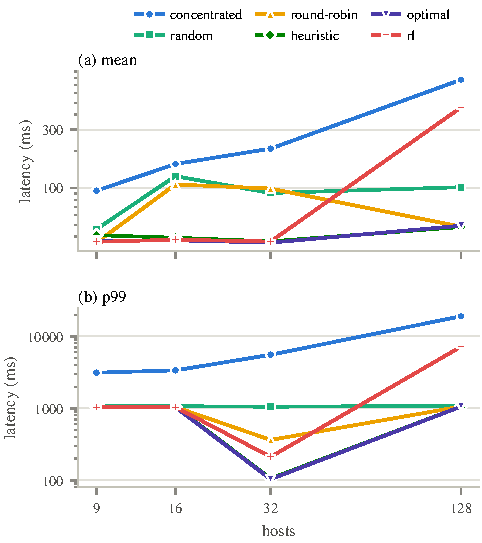
\includegraphics[width=\columnwidth]{figures/fig_latency_scale.pdf}
\caption{Per-call service latency vs.\ topology scale: (a) mean with cluster-bootstrap
95\% confidence intervals, (b) p95 (log axes). The 9-host point is the homogeneous
scenario (its \texttt{baseline} method, which exists only there, is omitted);
16/32/128 hosts are the scaled heterogeneous scenarios of
Tables~\ref{tab:scaled16}, \ref{tab:scaled32}, and~\ref{tab:scaled128}. The p95 panel
shows the degraded-host penalty that \texttt{round\_robin} and \texttt{random} pay at
16 and 32 hosts; \texttt{PPO} tracks the feature-aware methods until 128 hosts.}
\label{fig:latencyscale}
\end{figure}

\subsection{Mechanism Check: Latency vs.\ Backup Load}

Table~\ref{tab:backupload} pools service latency by \texttt{backup\_load} (the number of
primaries sharing a given backup), aggregated to one observation per
(run $\times$ backup) so that the thousands of correlated calls against a single heavily
loaded server count once rather than many times. Mean latency rises monotonically with
load in every scenario, isolating sharing itself, independent of which method produced
the sharing pattern, as the mechanism driving latency under contention. This is a
genuine architectural property of DEFT's unmodified single-threaded backup.

\begin{table}[t]
\centering
\caption{Service latency vs.\ backup load, one observation per (run $\times$ backup).}
\label{tab:backupload}
\resizebox{\columnwidth}{!}{%
\begin{tabular}{clrrr}
\toprule
Scenario & Load & $n$ units & Mean (ms) & 95\% CI \\
\midrule
\multirow{4}{*}{Homog.} & 1 & 354 & 45.23 & [44.60, 45.89] \\
 & 2 & 33 & 68.07 & [65.80, 70.35] \\
 & 3 & 15 & 96.94 & [90.51, 104.25] \\
 & 4 & 15 & 126.20 & [117.85, 135.44] \\
\midrule
\multirow{4}{*}{16-host} & 1 & 678 & 104.56 & [98.86, 110.46] \\
 & 2 & 21 & 107.14 & [100.41, 113.65] \\
 & 3 & 15 & 229.03 & [115.11, 349.47] \\
 & 9 & 15 & 190.79 & [181.37, 199.20] \\
\bottomrule
\end{tabular}}
\end{table}
\subsection{Scalability Trend: 32 Hosts}
\label{sec:scale32}

Figure~\ref{fig:latencyscale} plots mean and p95 across the full four-point scale sweep.
Table~\ref{tab:scaled32} reports the 32-host point, now run at the same protocol as
every other scale (5 context seeds $\times$ 3 trials, 200 calls/primary, burst 10)
rather than the reduced protocol used in an earlier version of this experiment; as
\S\ref{sec:p99} explains, that reduction was what produced a spurious order-of-magnitude
p99 improvement at this scale.

The 16-host finding holds at $2\times$ scale: \texttt{concentrated}, \texttt{heuristic},
\texttt{optimal}, and \texttt{PPO} again never route to a degraded host in any seed;
\texttt{round\_robin} hits one in 4 of 20 assignments, every seed.
Table~\ref{tab:scaled32-paired} gives the paired comparisons: \texttt{round\_robin}
again loses to the heuristic in all 15 paired runs ($+43.7$\,ms, $r = +1.000$,
$p_{\mathrm{Holm}} = 0.0009$), as do \texttt{random} ($+52.0$\,ms) and
\texttt{concentrated} ($+170.0$\,ms), while \texttt{optimal} and \texttt{PPO} remain
indistinguishable from it ($p_{\mathrm{Holm}} \ge 0.61$). Notably,
\texttt{round\_robin}'s degraded-host hit rate is not a random draw but a fixed
consequence of how Python's alphabetical host-name sort aligns with the degraded hosts;
\S\ref{sec:rl128} shows this coincidence flips at 128 hosts.

\begin{table}[t]
\centering
\caption{Scaled heterogeneous, 32 hosts (20 primaries, 4 degraded), 15 runs.}
\label{tab:scaled32}
\resizebox{\columnwidth}{!}{%
\begin{tabular}{lrrrr}
\toprule
Method & Mean (ms) & 95\% CI of mean & Median (ms) & p95 (ms) \\
\midrule
\texttt{concentrated} & 296.00 & [277.56, 315.07] & 8.19 & 1332.60 \\
\texttt{random} & 172.59 & [157.84, 187.04] & 79.51 & 338.52 \\
\texttt{round\_robin} & 163.39 & [160.25, 166.36] & 86.27 & 362.48 \\
\texttt{heuristic} & 121.39 & [116.33, 126.96] & 85.22 & 200.81 \\
\texttt{optimal} & 123.29 & [118.27, 129.49] & 87.42 & 221.41 \\
\texttt{PPO} & 130.38 & [122.57, 139.30] & 84.39 & 243.23 \\
\bottomrule
\end{tabular}}
\end{table}
\begin{table}[t]
\centering
\caption{32 hosts: paired comparisons against the heuristic.}
\label{tab:scaled32-paired}
\resizebox{\columnwidth}{!}{%
\begin{tabular}{lrrrl}
\toprule
Method vs.\ \texttt{heuristic} & $\Delta$ median (ms) & $r$ & $p_{\mathrm{Holm}}$ & Verdict \\
\midrule
\texttt{concentrated} & +169.97 & +1.000 & 0.0009 & significant \\
\texttt{random} & +52.02 & +1.000 & 0.0009 & significant \\
\texttt{round\_robin} & +43.69 & +1.000 & 0.0009 & significant \\
\texttt{optimal} & +3.81 & +0.100 & 0.7615 & n.s. \\
\texttt{PPO} & +15.28 & +0.400 & 0.6057 & n.s. \\
\bottomrule
\end{tabular}}
\end{table}
\subsection{Scalability Trend Continued: 128 Hosts}
\label{sec:rl128}

Table~\ref{tab:scaled128} reports the 128-host point at the same protocol as every other
scale. This is the only scale at which client-side retry behavior contributes measurably
to observed latency, and Table~\ref{tab:decomposition} separates the two components. For
every feature-aware method the client never retries at all and wall-clock time equals
backup service time exactly. For \texttt{concentrated}, by contrast, 3.53\% of calls
retry and \emph{19.6 of the 35.1\,s wall-clock p99 is the client's own exponential-backoff
sleep} rather than backup delay. Reporting the two fused, as our earlier harness did,
attributes the client's sleep constants to the server under test; the genuine service-time
p99 is 15.5\,s, itself a real and severe queueing pathology, but not the 35\,s the fused
number suggests.

\begin{table}[t]
\centering
\caption{128 hosts: backup service time vs.\ client retry wait. Only at this scale does client-side backoff contribute measurably; at 9/16/32 hosts no call retries.}
\label{tab:decomposition}
\resizebox{\columnwidth}{!}{%
\begin{tabular}{lrrrr}
\toprule
Method & Service p99 & Wall p99 & Retry wait & Calls retried (\%) \\
\midrule
\texttt{concentrated} & 15485.05 & 35081.66 & 19596.61 & 3.53 \\
\texttt{random} & 1434.86 & 1434.90 & 0.04 & 0.00 \\
\texttt{round\_robin} & 1189.76 & 1189.76 & 0.00 & 0.00 \\
\texttt{heuristic} & 1203.12 & 1203.12 & 0.00 & 0.00 \\
\texttt{optimal} & 1263.54 & 1263.54 & 0.00 & 0.00 \\
\texttt{PPO} & 7210.80 & 7281.93 & 71.13 & 0.27 \\
\bottomrule
\end{tabular}}
\end{table}
\textbf{Round-robin, heuristic, and optimal are indistinguishable at this scale.}
\texttt{round\_robin}'s mapping happens to hit zero degraded-host assignments at 128
hosts (the alphabetical-sort coincidence noted in \S\ref{sec:scale32}), so it is not
penalized here for the mechanism this scenario is designed to test. It, the heuristic
and the optimum are statistically indistinguishable ($p_{\mathrm{Holm}} \ge 0.66$).
Table~\ref{tab:scaled128-paired} gives the full comparison.
This is not a reversal of our core claim but its clearest illustration: round-robin's
outcome is uncontrolled, losing every paired run at 16 and 32 hosts and drawing level at
128 purely by naming coincidence, whereas heuristic and optimal avoid degraded hosts
\emph{by construction} regardless of scale, naming, or noise. \texttt{random}, which has
no such luck, remains significantly worse ($+46.6$\,ms, $r = +1.000$).

\textbf{PPO degrades sharply at this scale.} The learned policy is worse than the
heuristic by 145\,ms at the median run and loses all 15 paired runs ($r = +1.000$,
$p_{\mathrm{Holm}} = 0.0009$), with a p95 of 1197\,ms against the heuristic's 295\,ms.
Its median (96\,ms) is in fact the \emph{lowest} of any method, so the penalty is
concentrated in a tail: the policy places most primaries well and a minority disastrously.

\begin{table}[t]
\centering
\caption{Scaled heterogeneous, 128 hosts (80 primaries, 16 degraded), 15 runs.}
\label{tab:scaled128}
\resizebox{\columnwidth}{!}{%
\begin{tabular}{lrrrr}
\toprule
Method & Mean (ms) & 95\% CI of mean & Median (ms) & p95 (ms) \\
\midrule
\texttt{concentrated} & 536.87 & [503.12, 577.55] & 8.09 & 3424.71 \\
\texttt{random} & 214.96 & [200.43, 232.83] & 129.24 & 470.15 \\
\texttt{round\_robin} & 156.64 & [147.22, 166.78] & 117.53 & 277.70 \\
\texttt{heuristic} & 167.05 & [152.06, 189.09] & 127.45 & 294.72 \\
\texttt{optimal} & 189.25 & [153.21, 252.63] & 126.68 & 385.80 \\
\texttt{PPO} & 328.86 & [296.21, 368.31] & 96.46 & 1196.85 \\
\bottomrule
\end{tabular}}
\end{table}
\begin{table}[t]
\centering
\caption{128 hosts: paired comparisons against the heuristic.}
\label{tab:scaled128-paired}
\resizebox{\columnwidth}{!}{%
\begin{tabular}{lrrrl}
\toprule
Method vs.\ \texttt{heuristic} & $\Delta$ median (ms) & $r$ & $p_{\mathrm{Holm}}$ & Verdict \\
\midrule
\texttt{concentrated} & +360.55 & +1.000 & 0.0009 & significant \\
\texttt{random} & +46.57 & +1.000 & 0.0009 & significant \\
\texttt{round\_robin} & -4.25 & -0.300 & 0.6605 & n.s. \\
\texttt{optimal} & -2.48 & -0.133 & 0.6788 & n.s. \\
\texttt{PPO} & +145.28 & +1.000 & 0.0009 & significant \\
\bottomrule
\end{tabular}}
\end{table}
\textbf{What drives it.} The original \texttt{rl\_model\_scaled128} (400,000 timesteps,
\texttt{stable-baselines3}'s default entropy coefficient of 0 and a $[64,64]$ network)
converged to a near-degenerate policy, using only 1--5 distinct backups out of 80 and
funnelling almost every primary onto one host. Since PPO's entropy bonus is zero by
default, nothing discourages a policy from locking onto one action early once it looks
decent on average, compounded by a $[64,64]$ network's limited capacity to represent a
policy conditioned on which of 80 one-hot-encoded primaries is active. Two escalating
retraining attempts followed: an intermediate one (entropy 0.01, $[128,128]$, 600k
timesteps) that improved the spread only partially, and the fix that produced the
reported model (entropy 0.02, $[256,256]$, larger rollout and batch sizes, 1M timesteps).
Both are shipped as reproducible checkpoints.

The fixed policy avoids degraded hosts completely (zero degraded assignments across all
5 seeds) but still spreads the 80 primaries across far fewer backups than the heuristic
does, and it is that residual concentration which produces the tail in
Table~\ref{tab:scaled128}. The mechanism is visible in the reward: the health and
capacity terms label which hosts are bad and the network learns that signal, whereas
concentration is discouraged only implicitly, through the health/capacity decay, and
never by a direct anti-concentration term. Host-quality discrimination and
load-balancing precision are therefore acquired at different rates as the action space
grows. Reward shaping that penalizes load concentration directly is a natural way to
address this; we did not attempt it here, and leave a fuller study of RL for backup
selection in this setting to future work (\S\ref{sec:conclusion}).

\subsection{Cross-Algorithm Check: DQN}
\label{sec:dqn}

The load-balancing gap of \S\ref{sec:rl128} is measured on one algorithm, which leaves open
whether it reflects PPO or the problem formulation. To separate these we repeat the
evaluation with Deep Q-Networks (DQN)~\cite{mnih2015human}, a deliberately different design
point: off-policy with a replay buffer rather than on-policy, value-based rather than
actor-critic, and exploring by epsilon-greedy decay rather than an entropy bonus. DQN is
trained and evaluated through the same environment, reward, and inference path as PPO, so only the learning algorithm differs.

We score both policies \emph{structurally}, by degraded-host assignments, distinct backups
used, and maximum per-backup load (Table~\ref{tab:ppodqn}). These are properties of the
produced mapping rather than of RPC timing, which matters here for two reasons. First,
load-balancing precision is itself a structural property, so this measures the quantity in
question directly rather than through its latency consequence, and
Table~\ref{tab:backupload} has already established backup load as what drives latency under contention. Second, structural metrics are hardware-independent, so unlike per-call latency
they reproduce exactly on any machine.

\begin{table}[t]
\centering
\caption{PPO vs.\ DQN policy structure, 5 context seeds per scale. ``Distinct'' is the range
of distinct backups a policy assigns its primaries across seeds (higher is a wider spread),
``Peak'' the largest number of primaries placed on any one backup (lower is better), and
``Degraded'' the assignments landing on a deliberately degraded host, out of 5 seeds
$\times$ $|P|$.}
\label{tab:ppodqn}
\resizebox{\columnwidth}{!}{%
\begin{tabular}{llrrr}
\toprule
Scale & Algorithm & Distinct & Peak & Degraded \\
\midrule
\multirow{2}{*}{9-host} & PPO & 5--5 of 5 & 1--1 & 0/25 \\
 & DQN & 5--5 of 5 & 1--1 & 0/25 \\
\midrule
\multirow{2}{*}{16-host} & PPO & 10--10 of 10 & 1--1 & 0/50 \\
 & DQN & 9--10 of 10 & 1--2 & 0/50 \\
\midrule
\multirow{2}{*}{32-host} & PPO & 15--19 of 20 & 2--2 & 0/100 \\
 & DQN & 12--16 of 20 & 2--3 & 1/100 \\
\midrule
\multirow{2}{*}{128-host} & PPO & 24--30 of 80 & 9--28 & 0/400 \\
 & DQN & \textbf{1--3 of 80} & \textbf{45--80} & \textbf{172/400} \\
\bottomrule
\end{tabular}}
\end{table}

\textbf{Up to 32 hosts the two algorithms behave alike.} Both spread across nearly every
available backup at 9 and 16 hosts, and at 32 hosts DQN stays within a few backups of PPO at
a comparable peak load, with a single incidental degraded-host assignment. Reaching that
required the same class of intervention PPO needed at 128 hosts: with library-default
settings DQN collapsed to 2--4 distinct backups of 20, and widening exploration (exploration
fraction $0.5 \rightarrow 0.7$, final epsilon $0.05 \rightarrow 0.15$), enlarging the replay
buffer ($50\text{k} \rightarrow 100\text{k}$), and training longer
($100\text{k} \rightarrow 150\text{k}$ steps) recovered the spread reported here.

\textbf{At 128 hosts DQN concentrates far more sharply than PPO.} It funnels the 80 primaries
onto 1--3 distinct backups with up to 80 primaries on a single host, and routes 172 of 400
assignments onto degraded hosts. PPO, with its entropy- and capacity-scaled configuration,
avoids degraded hosts entirely in the same comparison while still spreading across only
24--30 backups, against the heuristic's 74--76 at a maximum load of 2 (\S\ref{sec:rl128}).

\textbf{What this establishes.} Two algorithms that differ in exploration mechanism, policy
representation, and update rule both concentrate load as the action space grows, and both
respond to the same widened-exploration remedy. The behavior is therefore better attributed
to the problem formulation, in particular a reward that labels host quality explicitly but
discourages concentration only implicitly, than to any single algorithm. It also sharpens the
practical reading of \S\ref{sec:rl128}: the deterministic heuristic reaches a wider spread
than either learned policy with no training, no per-scale tuning, and no exposure to this
failure mode.

\subsection{Heuristic Weight Sensitivity and Decay Calibration}
\label{sec:weights}

\S\ref{sec:methods} fixes the multi-criteria heuristic's scoring weights at
$(w_h, w_k, w_\ell, w_d) = (0.35, 0.35, 0.20, 0.10)$ and its load-decay mechanics
($\mathrm{cap} \mathrel{-}= 20$; $\mathrm{health} \mathrel{*}= 0.95$) by intuition. To
show these are principled rather than ad hoc, we run a systematic sensitivity sweep: 287
weight configurations (286 points on a 0.1-step grid over the 4-simplex, plus the exact
published default, which does not fall on that grid), each evaluated \emph{structurally}
(degraded-host hit rate, maximum per-backup load, and distinct backups used) across
the real 9-host DEFT topology and the synthetic 16/32/128-host topologies, 5 context-seed
draws each. This sweep requires no RPC calls (it evaluates
\texttt{backup\_selector.select\_backups} directly against each synthetic resource draw),
so it is exact and reproducible rather than subject to RPC-timing noise.

\textbf{Degraded-host avoidance is essentially weight-independent.} All 287 configurations,
at all four topologies (1{,}148 configuration-topology pairs total), achieved 0\%
degraded-host usage, including the extreme case of weighting 100\% on hops alone. This
is a direct consequence of how starkly the artificially-degraded hosts are constructed
relative to normal ones (health 0.05 vs.\ 0.5--1.0; capacity fraction $\approx 0.033$
vs.\ $\approx 0.4$--1.0): the gap is large enough that even a weight vector with zero net
discriminative power still favors a non-degraded candidate on tie-break. The heuristic's
degraded-host-avoidance guarantee is therefore robust to the exact weight choice, not a
fragile artifact of the specific published weights.

\textbf{Load-balancing quality is highly weight-sensitive, and its principal lever is the
capacity decay term.} Across the sweep, maximum per-backup load ranges from perfect (max
load of 1 primary/backup, achieved whenever the capacity weight is nonzero and
health/latency/hops are near zero) to severe (up to 79 of 80 primaries sharing one backup
at 128 hosts, when capacity and health weights are both zero). The capacity term,
realised as the flat $-20$ decrement applied to a chosen backup's remaining capacity after
each assignment, is the dominant load-balancing lever: even a small nonzero capacity
weight alone reaches near-optimal balance at every scale tested. The health decay
($\times 0.95$ per assignment) is a weaker lever toward the same end, and the latency and
hops terms contribute essentially nothing to load-balancing in the topologies tested,
since every backup-eligible host is exactly two hops from any primary via the shared hub
and so normalizes to zero. This directly addresses whether the decay mechanics are
arbitrary: they \emph{are} the mechanism by which load spreads across the pool, and the
sweep shows the $-20$ capacity decrement specifically is what drives it.

\begin{table}[t]
\centering
\caption{Published default weights ($w_h{=}0.35$, $w_k{=}0.35$, $w_\ell{=}0.20$,
$w_d{=}0.10$) vs.\ the best achievable (max load $=1$) at each scale, 5-seed average.}
\label{tab:weights}
\resizebox{\columnwidth}{!}{%
\begin{tabular}{lrrrr}
\toprule
Scale & Default max load & Best max load & Default backups used & Max possible \\
\midrule
9-host (real) & 1.40 & 1.00 & 4.60 & 5 \\
16-host & 1.40 & 1.00 & 9.40 & 10 \\
32-host & 2.00 & 1.00 & 18.00 & 20 \\
128-host & 2.00 & 1.00 & 74.80 & 80 \\
\bottomrule
\end{tabular}}
\end{table}

\textbf{The published default is a principled, near-optimal choice}
(Table~\ref{tab:weights}): at every scale it lands within one unit of the achievable
max-load optimum and uses 90--94\% of the maximum possible distinct backups. Sorted by
(degraded-rate, max-load), the default configuration ranks 151st--187th of the 287 grid
points across scales, a position that looks middling only because so many configurations
tie at the max-load-of-1 ceiling (any configuration with a nonzero capacity weight tends to
reach it); the default is a small, practically immaterial distance from that ceiling, not
meaningfully behind it. The honest limitation this sensitivity analysis surfaces is not
that the published weights or decay constants are poorly chosen, but that two of the four
terms (latency, hops) carry negligible practical weight in the uniform-hop synthetic
topologies used here, a consequence of the RPC-isolation testbed (\S\ref{sec:threats})
rather than of the scoring design itself, which would plausibly matter more on a real
bandwidth-constrained, variable-latency network.

\textbf{The decay constants themselves are a characterized, well-behaved lever, not an ad
hoc choice.} To address the load-decay mechanics directly, we additionally sweep both
constants (the capacity decrement over $\{5,10,20,40,80\}$ and the health-decay factor over
$\{0.80,0.90,0.95,0.99,1.00\}$) with the scoring weights fixed, 5 seeds per topology (100
decrement$\times$decay$\times$topology cells). Two properties hold. First,
\emph{degraded-host avoidance is entirely decay-independent}: 0 of the 100 cells routed any
primary to a degraded host, confirming the safety guarantee comes from the scoring, not from
decay tuning. Second, load-balancing is a \emph{smooth, monotone} function of both constants:
holding the health decay at its published 0.95, raising the capacity decrement through
$5, 10, 20, 40, 80$ lowers mean maximum per-backup load through
$2.60, 2.00, 2.00, 1.00, 1.00$ (identical at 32 and 128 hosts), and a stronger health decay
moves it the same way. The published decrement of 20 is thus a deliberately conservative
operating point, within one unit of the perfect-spread optimum, that leaves a small, bounded
amount of load-balancing unclaimed rather than spreading maximally aggressively, which on a
pool with finer non-degraded quality variation could trade host quality for balance. The
published $(20, 0.95)$ is therefore a principled choice on a monotone response surface, not
an arbitrary constant.

\subsection{Decentralized Hash Baselines, a Fairer Round-Robin, and Topology Diversity}
\label{sec:hrw}

We broaden the baseline set along three axes the load-balancing and distributed-storage
literature would expect, and re-examine the findings structurally (degraded-host hits and
maximum per-backup load, 5-seed average, no RPC calls) in the heterogeneous scenarios where
host quality differs (Table~\ref{tab:hrw}).

\textbf{Decentralized hash placement (HRW and consistent hashing).} We add three
decentralized baselines in the style well established in distributed storage
(CRUSH~\cite{weil2006crush}, Dynamo~\cite{decandia2007dynamo}): plain rendezvous hashing
(\texttt{hrw}), health/capacity-weighted rendezvous hashing (\texttt{weighted\_hrw}), and
Dynamo-style weighted consistent hashing (\texttt{weighted\_chash}). Plain HRW is
health/capacity-unaware, and like round-robin its degraded-host exposure is uncontrolled:
it routes primaries to degraded hosts at 16 and 128 hosts and misses them at 32 only by hash
coincidence. Both \emph{weighted} variants avoid degraded hosts entirely (0 across all
scales), confirming that \emph{quality-awareness, not centralization, is what buys
degraded-host avoidance}. However, both are coordination-free (each primary hashes
independently, with no load penalty propagated between assignments), so they spread load
only statistically: mean maximum per-backup load is 3.0/3.6/2.2 (weighted HRW) and
2.8/3.0/3.2 (weighted consistent hashing) at 16/32/128 hosts, against the greedy heuristic's
1.4/2.0/2.0 and the Hungarian optimum's 1.0. A single coordinated greedy pass therefore
load-balances materially tighter than \emph{either} decentralized weighted-hash family at
equal degraded-host avoidance, and the exact assignment is tighter still.

\textbf{A fairer round-robin.} The deterministic round-robin's degraded-host exposure
depends on Python's alphabetical host-name sort, which happens to miss the degraded range at
128 hosts (\S\ref{sec:scale32}). Adding a randomized-offset round-robin (\texttt{rr\_random})
removes that artifact: with a random starting offset it hits degraded hosts at \emph{every}
scale (1.2/2.6/10.8 primaries at 16/32/128 hosts, tracking the degraded fraction),
confirming that the deterministic variant's apparent 128-host safety was pure naming
coincidence, and that any quality-blind load-spreader is exposed to degraded hosts in
proportion to how many there are. This strengthens rather than weakens the core claim: the
feature-aware methods avoid degraded hosts \emph{by construction} at every scale, a guarantee
no round-robin variant offers.

\textbf{Topology diversity.} To test whether the findings depend on the single-hub star, we
repeat the comparison on multi-hub topologies (three hubs in a line, hosts distributed across
them, so host-to-host hop-count and latency now vary). The structural outcome is unchanged:
at 16-host/3-hub and 32-host/3-hub the heuristic still avoids degraded hosts entirely at a
maximum load of 1.4 and 2.0 (identical to the single-hub stars), the weighted-hash baselines
still avoid degraded hosts but spread loosely (max load $\approx 3$), and the fair
round-robin still hits degraded hosts (1.2 and 2.6). Because degraded-host avoidance and
load-balancing are driven by host \emph{quality} rather than graph \emph{shape}, the core
findings are robust to topology structure; a fuller sweep over irregular, multi-hub, and
uneven-fan-out graphs remains future work (\S\ref{sec:threats}).

\begin{table}[t]
\centering
\caption{Decentralized hash baselines and a fairer round-robin vs.\ the feature-aware
methods, 5-seed average, heterogeneous star scenarios (multi-hub results are identical; see
text). ``Deg.'' = mean primaries routed to a degraded host (lower is better); ``Load'' = mean
max per-backup load (lower is a tighter spread).}
\label{tab:hrw}
\resizebox{\columnwidth}{!}{%
\begin{tabular}{lcccccc}
\toprule
& \multicolumn{2}{c}{16-host} & \multicolumn{2}{c}{32-host} & \multicolumn{2}{c}{128-host}\\
\cmidrule(lr){2-3}\cmidrule(lr){4-5}\cmidrule(lr){6-7}
Method & Deg. & Load & Deg. & Load & Deg. & Load \\
\midrule
round\_robin & 2.0 & 1.0 & 4.0 & 1.0 & 0.0 & 1.0 \\
rr\_random & 1.2 & 1.0 & 2.6 & 1.0 & 10.8 & 1.0 \\
hrw & 2.0 & 3.0 & 0.0 & 3.0 & 9.0 & 2.0 \\
weighted\_hrw & 0.0 & 3.0 & 0.0 & 3.6 & 0.0 & 2.2 \\
weighted\_chash & 0.0 & 2.8 & 0.0 & 3.0 & 0.0 & 3.2 \\
heuristic & \textbf{0.0} & \textbf{1.4} & \textbf{0.0} & \textbf{2.0} & \textbf{0.0} & \textbf{2.0} \\
optimal & 0.0 & 1.0 & 0.0 & 1.0 & 0.0 & 1.0 \\
\bottomrule
\end{tabular}}
\end{table}

\subsection{Selection Overhead}

``Elastic scaling'' requires the selection algorithm itself to be fast: a method that
matches the optimal bound on placement quality but takes seconds to compute is a
materially worse deployment story than one that is comparably fast. Table~\ref{tab:overhead}
reports the mean wall-clock time to compute one full mapping, across all four topology
sizes (30 repeats each, first call excluded as warmup), and
Figure~\ref{fig:overhead} plots the same data on log--log axes. Even the slowest method
computes a full 128-host mapping in about 60\,ms (\texttt{PPO}, 61.6\,ms mean), and every
non-learned method in roughly 10\,ms or less, negligible relative to any realistic
failure-detection interval
(typically hundreds of milliseconds to seconds in NF failure-recovery
literature~\cite{gill2011understanding,potharaju2013demystifying}). \texttt{PPO} is
consistently slowest (one PPO forward pass per primary, plus framework call overhead);
its jump at 128 hosts is the direct cost of the wider $[256,256]$ network needed to fix
the policy collapse described in \S\ref{sec:rl128}, on top of the growth in primary
count.
\texttt{heuristic} and \texttt{optimal} grow roughly linearly/superlinearly with host
count (the Hungarian algorithm is $O(n^3)$) but remain near 10\,ms at 128 hosts. None of
the feature-aware methods introduce a
selection-latency cost that would offset their placement-quality advantage in practice.

\begin{table}[t]
\centering
\caption{Selection overhead (ms) per full mapping computation, mean of 30 repeats
(first call excluded as warmup).}
\label{tab:overhead}
\resizebox{\columnwidth}{!}{%
\begin{tabular}{lrrrr}
\toprule
Method & 9 hosts & 16 hosts & 32 hosts & 128 hosts \\
\midrule
\texttt{concentrated} & 0.006 & 0.021 & 0.035 & 0.600 \\
\texttt{random} & 0.028 & 0.043 & 0.054 & 0.567 \\
\texttt{round\_robin} & 0.005 & 0.007 & 0.009 & 0.055 \\
\texttt{heuristic} & 0.050 & 0.145 & 0.600 & 10.277 \\
\texttt{optimal} & 0.081 & 0.271 & 0.860 & 9.968 \\
\texttt{PPO} & 6.345 & 5.065 & 10.605 & 61.636 \\
\texttt{DQN} & 1.404 & 6.209 & 6.217 & 40.080 \\
\bottomrule
\end{tabular}}
\end{table}

\begin{figure}[t]
\centering
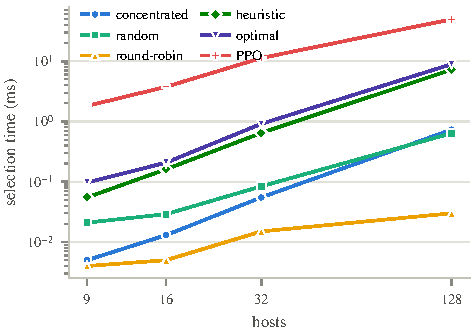
\includegraphics[width=\columnwidth]{figures/fig_overhead.pdf}
\caption{Selection overhead per full mapping computation (log--log axes; data of
Table~\ref{tab:overhead}). Even the slowest method (\texttt{PPO}, 49.6\,ms at 128
hosts) remains well below realistic failure-detection intervals.}
\label{fig:overhead}
\end{figure}

\subsection{Throughput and Failure Rate}

Tables~\ref{tab:throughput9} and~\ref{tab:throughput16} complement service latency with
the other two metrics DEFT's original evaluation reports: throughput and packet drop. We
measure each primary's burst workers for a fixed 3-second wall-clock window (rather than
a fixed call count) and report successful calls/second and the percentage of calls that
fail even after retry, with one observation per run and the same paired analysis as
\S\ref{sec:stats}. This testbed is RPC-level (TCP), not DEFT's own packet-level
input-buffer-overflow mechanism, which requires the Mininet/stamped-packet path this
testbed deliberately bypasses; ``failure rate'' here is evidence of the same underlying
phenomenon (an overloaded backup failing to keep up with demand), not a literal
reproduction of DEFT's packet-drop metric.

\begin{table}[t]
\centering
\caption{Throughput/failure rate, homogeneous scale (15 runs).}
\label{tab:throughput9}
\resizebox{\columnwidth}{!}{%
\begin{tabular}{lrrr}
\toprule
Method & Throughput (calls/s) & 95\% CI & Failure rate (\%) \\
\midrule
\texttt{baseline} & 523.20 & [440.78, 617.89] & 1.021 \\
\texttt{concentrated} & 530.02 & [437.56, 634.27] & 1.781 \\
\texttt{random} & 520.53 & [436.37, 613.89] & 0.797 \\
\texttt{round\_robin} & 547.09 & [442.24, 669.62] & 0.282 \\
\texttt{heuristic} & 570.67 & [473.06, 683.80] & 0.480 \\
\texttt{optimal} & 549.62 & [453.67, 661.73] & 0.227 \\
\texttt{PPO} & 541.69 & [461.73, 630.05] & 0.315 \\
\bottomrule
\end{tabular}}
\end{table}

At homogeneous scale we draw no conclusion from throughput. Each method contributes only
15 aggregate measurements, against the tens of thousands of individual calls behind each
latency test, and \emph{none} of the 21 pairwise comparisons survives Holm-Bonferroni
correction; the confidence intervals overlap almost completely. Aggregate throughput
here is dominated by background system load rather than by the mapping under test.
Failure rate is the one consistent signal: \texttt{concentrated}'s 1.78\% is the highest
of any method, while the feature-aware methods stay at 0.23--0.48\%.

\begin{table}[t]
\centering
\caption{Throughput/failure rate, 16-host scaled scenario (15 runs).}
\label{tab:throughput16}
\resizebox{\columnwidth}{!}{%
\begin{tabular}{lrrr}
\toprule
Method & Throughput (calls/s) & 95\% CI & Failure rate (\%) \\
\midrule
\texttt{concentrated} & 543.84 & [477.84, 616.58] & 5.821 \\
\texttt{random} & 688.84 & [626.53, 757.76] & 1.224 \\
\texttt{round\_robin} & 733.49 & [677.93, 795.25] & 0.428 \\
\texttt{heuristic} & 752.64 & [689.98, 821.42] & 0.480 \\
\texttt{optimal} & 740.11 & [691.78, 790.83] & 0.264 \\
\texttt{PPO} & 780.96 & [721.91, 846.84] & 0.321 \\
\bottomrule
\end{tabular}}
\end{table}

At 16 hosts, contention is severe enough that one part of the throughput picture becomes
robust. \texttt{concentrated} is significantly out-thoughput by \emph{every} other
method ($r \in [-1.000, -0.900]$, all $p_{\mathrm{Holm}} \le 0.019$), and its failure
rate (5.82\%) is an order of magnitude above the feature-aware methods'
(0.26--0.48\%). Gross load concentration is therefore visible from the throughput side,
not only from service latency.

The degraded-host effect is a subtler matter, and the honest characterization is that
aggregate throughput resolves it only partially. \texttt{PPO} does significantly
out-throughput \texttt{round\_robin} ($r = -0.933$, $p_{\mathrm{Holm}} = 0.0047$),
consistent with \texttt{round\_robin} pairing 2 of its 10 primaries with a degraded
backup in every seed; yet neither \texttt{heuristic} nor \texttt{optimal} reaches
significance against \texttt{round\_robin} ($p_{\mathrm{Holm}} \ge 0.86$) despite
avoiding degraded hosts exactly as \texttt{PPO} does. The mechanism explains the
fragility: only 2 of \texttt{round\_robin}'s 10 primaries are actually paired with a
degraded backup, and their reduced individual throughput is averaged into the other 8
primaries' normal throughput at the aggregate level, leaving a signal small enough that
run-to-run noise decides the verdict. Service latency is dominated by exactly the slow
calls that throughput's mean-based aggregation smooths over, and resolves the same effect
consistently at every scale we tested. This is why we treat latency as the primary metric
throughout and throughput as corroborating rather than replacing evidence: throughput
reliably resolves gross contention, but only marginally resolves the finer degraded-host
effect that this paper is actually about.

\section{Threats to Validity}
\label{sec:threats}

\textbf{RPC-isolation testbed, not the physical Mininet network (the primary external-validity
gap).} As described in \S\ref{sec:methodology}, we exercise DEFT's real backup RPC server
directly rather than over a physical/emulated network path, after the available Mininet
environment could not provide a genuine bandwidth constraint for contention to manifest
against. This gives a direct, reproducible measurement of the contention mechanism at the
cost of not validating full end-to-end network behavior (switching, real link bandwidth,
packet loss) and, in particular, DEFT's own packet-level, controller-integrated data path.
A packet-level evaluation over a working OVS/SDN-controller Mininet fabric, against which
the RPC-level failure rate could be cross-checked with DEFT's native packet-drop metric, is the most important remaining validation, and we treat the present study as isolating the backup-selection mechanism rather than certifying end-to-end network performance.

\textbf{Single physical machine.} All ``hosts'' are OS processes on one machine;
OS-level scheduling noise is a real, visible component of measured service latency.
Multi-seed aggregation and the paired run-level design mitigate but do not eliminate this.

\textbf{Synthetic resource values and injected heterogeneity.} Health, capacity, CPU, and
storage availability are drawn from the configured ranges of \S\ref{sec:methods}, and
heterogeneity is injected via a fixed $+50$\,ms per-call delay and pinned degraded resource
numbers, not measured from real workload telemetry; absolute magnitudes are therefore
illustrative rather than calibrated. \S\ref{sec:methods} maps each synthetic feature to the
real NFV telemetry it stands in for, but validating the selection against that live telemetry
remains future work, and limits the ecological validity of the absolute (though not the
relative) results.

\textbf{RL configuration scales with the action space.} A PPO agent's observation and action
space is fixed to a given host count, so a differently-sized topology is served by its own
trained model, and, as \S\ref{sec:rl128} shows, the exploration and network-capacity budget
must grow with the action space (the defaults that suffice at 16 and 32 hosts require scaling
up at 128). We report the resulting behavior and leave reward shaping against load
concentration, and a broader study of RL for this problem, to future work. For
reproducibility, the reported RL numbers describe the specific released checkpoints;
retraining under a different \texttt{stable-baselines3}/\texttt{PyTorch} version or host count yields a different but qualitatively similar policy. The same applies to DQN, which
additionally required its own exploration widening at 32 hosts (\S\ref{sec:dqn}).

\textbf{Deterministic round-robin's degraded-host exposure is coincidental.} Its exposure depends on how Python's alphabetical host-name sort aligns with the degraded hosts (hitting them at 16/32 hosts, missing at 128); the randomized-offset variant of \S\ref{sec:hrw}
confirms the exposure is real and proportional to the degraded fraction. This does not affect
the load-bearing claim that heuristic and optimal avoid degraded hosts by construction at
every scale, and that PPO does so empirically at every scale tested, which no round-robin
variant guarantees.

\textbf{The transport, not the replication protocol, shapes the latency tail.} As
\S\ref{sec:p99} establishes, DEFT's backup is an HTTP/1.0
\texttt{SimpleXMLRPCServer} with a five-deep accept backlog, so every replication call
opens a fresh TCP connection and the tail is quantized by the kernel's SYN-retransmission
timer. This is a real property of the implementation under test, not a harness artifact,
but it is a property of its \emph{transport}: a production replication path over gRPC,
RDMA, or a DPDK ring would exhibit queueing behavior of an entirely different shape. The
\emph{relative} ordering of selection methods, which is what this paper claims, is driven
by how many primaries share a backup and is robust to this; the absolute latency
magnitudes are not transferable.

\textbf{Absolute latencies are not reproducible across executions.} Ephemeral-port
TIME\_WAIT pressure shifts the mean of every method by of order 17\,ms between otherwise
identical executions (\S\ref{sec:p99}). The paired design cancels this, since the drift
is common-mode, but it sets a resolution floor: we make no claim about differences of a
few milliseconds, and two such claims that appeared significant in a single execution did
not survive replication (\S\ref{sec:p99}, \S\ref{sec:scale32}).

\textbf{Scale sweep is four points, not a continuous curve.} All four are now run at an
identical protocol and harness version, but a continuous sweep would be needed for a
rigorous asymptotic scalability claim.

\textbf{Topology diversity is partially, not exhaustively, covered.} Beyond the single-hub
stars, we evaluate multi-hub topologies (\S\ref{sec:hrw}), where host-to-host hop-count and
latency vary, and the structural findings are unchanged, because degraded-host avoidance
and load-balancing are driven by host quality rather than graph shape. Our context-seed sweep
still varies only synthetic \emph{resource} draws per seed, however; the graph shapes tested
(single- and multi-hub) remain regular, and genuinely irregular graphs (uneven fan-out,
heterogeneous hub connectivity, real datacenter topologies) are untested. A fuller sweep over
such graphs, together with the continuous scale sweep noted above, would strengthen the
generalization claim.

\textbf{Two analyses are evaluated structurally rather than by measured latency.} The
weight and decay sweeps (\S\ref{sec:weights}) and the PPO-vs-DQN comparison
(\S\ref{sec:dqn}) both report properties of the produced mapping (degraded-host
assignments, maximum per-backup load, distinct backups used) instead of per-call RPC
latency. This keeps them exact, hardware-independent, and cheap enough to sweep 287 configurations, and it measures load-balancing precision directly rather than through its latency consequence; our mechanism check (Table~\ref{tab:backupload}) establishes that backup load is what drives latency under contention. The cost is that neither the ranking
of weight configurations nor DQN's latency under contention has been verified end to end
against measured latency alongside the other methods.

\section{Conclusion and Future Work}
\label{sec:conclusion}

Every major NF state-replication system we surveyed (OpenNF, Split/Merge, StatelessNF,
S6, Pico Replication, FTMB, REINFORCE, and DEFT) does not treat backup-node assignment as a decision with measurable consequences. We have closed this gap concretely with iDEFT, designing and rigorously evaluating three backup-selection
strategies (an exact Hungarian-optimal bound, a multi-criteria heuristic, and a PPO
policy) against DEFT's own static mapping and three naive baselines, by driving DEFT's
real, unmodified 2PC implementation under controlled contention across four topology
scales with statistically rigorous, multi-seed testing. Feature-aware methods reliably
avoid degraded backup hosts and substantially reduce mean and p95 service latency once
hosts differ in quality: at both 16 and 32 hosts the greedy heuristic beats blind
round-robin in every one of fifteen paired runs ($r = 1.00$,
$p_{\mathrm{Holm}} \le 0.0012$), while remaining statistically indistinguishable from the
Hungarian optimum at every scale we tested. Reinforcement learning (PPO) matches this performance up to 32
hosts and, at 128 hosts, avoids degraded hosts completely while its load-balancing precision
is lower than the heuristic's at that scale. A cross-algorithm check with DQN
reproduces that concentration behavior at scale, and more sharply, under the same
widened-exploration remedy, which attributes the gap to the problem formulation rather than
to one algorithm. We report this measured behavior and leave a
fuller study of RL for backup-node selection in this setting, including reward shaping that
directly penalizes load concentration, to future work. A systematic sensitivity analysis
over the heuristic's scoring weights and decay mechanics further shows that its
degraded-host-avoidance guarantee holds across the entire weight space tested, that its
load-balancing quality is governed almost entirely by the remaining-capacity term (whose
$-20$ decrement is the load-spreading mechanism), and that the published default weighting is a near-optimal, non-fragile choice, so the heuristic's calibration is principled, not
ad hoc.

We also report, as a methodological result, what this testbed cannot measure. Because
DEFT's backup server closes every connection, the per-call latency tail is quantized by
the kernel's TCP SYN-retransmission timer rather than by queueing, which makes p99
unusable as a latency metric here; and ephemeral-port pressure shifts absolute latencies
between otherwise identical executions by more than most of the differences one might
wish to claim. A run-level paired design, in which the independent unit is an execution
rather than an individual RPC call, absorbs both and is what allows the surviving claims
to be stated with confidence. We recommend it, and two independent replications per
configuration, for anyone evaluating placement policies on a comparable harness.

Future work includes: reward shaping that directly penalizes load concentration for the
RL policy at large scale; validating these findings over a physical or emulated network
path with genuine bandwidth constraints, and over a production-grade asynchronous
transport (gRPC, RDMA) whose queueing behavior differs in kind from XML-RPC's; extending
the multi-seed evaluation to vary topology structure, not just resource values; and a
continuous scalability sweep across an uninterrupted range of host counts.

\section*{Acknowledgment}
This work builds directly on the DEFT system~\cite{shahriyar2023deft} and its publicly
available implementation.

\bibliographystyle{IEEEtran}
\bibliography{references}

\end{document}
